\documentclass[sigconf]{webmedia}
%webmeda.cls is adapted from acmart.cls for use in Proceedings of the Brazilian Symposium on Multimedia and the Web (WebMedia)

%%
%% \BibTeX command to typeset the BibTeX logo in the docs
\AtBeginDocument{%
  \providecommand\BibTeX{{%
    \normalfont B\kern-0.5em{\scshape i\kern-0.25em b}\kern-0.8em\TeX}}}

\settopmatter{printacmref=false, printfolios=false}

%% Choose the appropriate event.
\setevent{webmedia}
\proceedingsDetails[WebMedia’2025]{Proceedings of the Brazilian Symposium on Multimedia and the Web}{2025}{Rio de Janeiro, Brazil}
\ISSN{2966-2753}

\usepackage{booktabs}
\usepackage{graphicx}
\graphicspath{{figuras/}{sample/}}

\begin{document}

\title{Classificação Automática da Dificuldade de Questões de Programação Utilizando Aprendizado de Máquina e LLMs}

\author{Carlos Eduardo Pereira Oliveira - 116233}
\email{carlos.oliveira1@ufv.br}
\affiliation{%
  \institution{Universidade Federal de Viçosa}
  \city{Viçosa}
  \country{Brasil}
}

\author{Luis Felipe Martins Pereira - 112710}
\email{luis.f.pereira@ufv.br}
\affiliation{%
  \institution{Universidade Federal de Viçosa}
  \city{Viçosa}
  \country{Brasil}
}
\renewcommand{\shortauthors}{Oliveira e Pereira}

\begin{abstract}
Este trabalho investiga se o nível de dificuldade de uma questão de programação pode ser inferido automaticamente apenas a partir do enunciado textual. Comparamos duas granularidades de rótulo (cinco níveis, derivados diretamente das avaliações dos alunos, e três níveis, obtidos colapsando as extremidades) e, com base no ganho consistente de precisão observado experimentalmente, adotamos \textbf{três níveis} como configuração final do sistema. A metodologia foi aplicada em duas bases distintas para permitir comparação direta: o \textbf{INF110} (Universidade Federal de Viçosa, 80 questões rotuladas pelos alunos) e o \textbf{Neps Academy} (1.333 questões rotuladas por juiz). Sobre representações TF-IDF, comparamos quatro famílias de modelos clássicos --- Regressão Logística, KNN, SVM linear e Random Forest --- em validação cruzada estratificada, com prevenção explícita de vazamento de informação. Os melhores resultados foram F1-macro $0{,}47$ (INF110, três níveis) e $0{,}60$ (Neps, três níveis), contra $0{,}30$ e $0{,}43$ na escala de cinco níveis. Um LLM servido pela plataforma \textbf{Groq} foi integrado em três papéis (\textit{baseline} de classificação, gerador de explicações e extrator de conceitos), e o pipeline foi encadeado em uma etapa de inferência que, dada uma questão nova, prevê sua dificuldade, identifica conceitos e recomenda exercícios semelhantes do catálogo. O classificador Random Forest treinado no Neps em três níveis é o que alimenta a ferramenta em uso prático.
\end{abstract}

\keywords{aprendizado de máquina, classificação de texto, processamento de linguagem natural, TF-IDF, LLMs, dificuldade de questões de programação}

\maketitle

\section{Introdução}

A classificação automática da dificuldade de questões de programação é um problema relevante em contextos educacionais, como plataformas de ensino e sistemas de recomendação de exercícios. A capacidade de estimar automaticamente o nível de dificuldade pode auxiliar tanto alunos quanto professores na organização do processo de aprendizagem, na montagem de listas balanceadas e na personalização de trilhas de estudo.

A principal pergunta que orientou o trabalho foi: \textit{é possível inferir automaticamente o nível de dificuldade de uma questão de programação apenas a partir de seu enunciado textual?} Para respondê-la, tratamos a tarefa como um problema de classificação supervisionada e a estudamos sobre duas bases reais: uma com dificuldade percebida pelos alunos e outra com dificuldade atribuída por juiz.

As principais contribuições deste trabalho são:
\begin{itemize}
  \item um \textit{pipeline} reprodutível e modular que vai da ingestão dos dados brutos à avaliação dos modelos, com configuração centralizada e suporte a múltiplas fontes de dados no mesmo arcabouço;
  \item uma comparação direta de duas granularidades de rótulo (cinco e três níveis) sobre duas bases (INF110 e Neps Academy), que justifica empiricamente a escolha por três níveis como configuração final;
  \item a comparação de quatro famílias de modelos clássicos sobre representações TF-IDF, com validação cruzada estratificada, busca de hiperparâmetros e prevenção explícita de vazamento de informação;
  \item a integração de um LLM (via plataforma \textbf{Groq}, com cliente OpenAI-compatível intercambiável por configuração) em três papéis estratégicos: \textit{baseline} de classificação, explicador e extrator de conceitos; e
  \item uma etapa de inferência integrada que, para uma questão nova, prevê a dificuldade (ML), identifica conceitos (LLM) e recomenda exercícios semelhantes por conceitos em comum e dificuldade compatível, funcionando como a ferramenta em uso prático.
\end{itemize}

\section{Trabalhos Relacionados}

A representação de textos por TF-IDF (\textit{Term Frequency--Inverse Document Frequency}) é uma técnica consolidada em recuperação de informação e classificação de texto~\cite{salton1988}, por ponderar termos de acordo com sua frequência local e raridade no corpus. Sobre essas representações, modelos clássicos de aprendizado de máquina são amplamente empregados: a classificação por vizinhos mais próximos~\cite{coverhart1967}, as máquinas de vetores de suporte~\cite{cortes1995} e as florestas aleatórias~\cite{breiman2001} figuram entre as abordagens mais robustas para dados esparsos, ao lado de métodos lineares. Toda a implementação apoiou-se em bibliotecas maduras do ecossistema Python, em especial o \texttt{scikit-learn}~\cite{pedregosa2011} e o \texttt{NLTK}~\cite{bird2009}.

Mais recentemente, Grandes Modelos de Linguagem (LLMs) têm sido aplicados a tarefas de compreensão textual em cenários de poucos exemplos (\textit{few-shot}), tornando-se candidatos naturais tanto como \textit{baselines} fortes quanto como ferramentas de extração de conhecimento. A estimativa automática de dificuldade, especificamente, é um problema desafiador porque a dificuldade percebida depende não só do texto, mas de conhecimentos prévios e habilidades do solucionador, o que motiva o uso combinado de representações clássicas e semânticas.

\section{Materiais e Métodos}

\subsection{Bases de Dados}
\label{sec:bases}

O trabalho utiliza \textbf{duas bases distintas} por escolha metodológica: uma reflete a dificuldade \emph{subjetiva} (percepção real dos alunos), a outra reflete a dificuldade \emph{objetiva} (juízo profissional). Estudar as duas em paralelo permite separar o que é característica do sinal textual do que é ruído de rótulo. Aplicamos exatamente a mesma metodologia a ambas para permitir comparação direta:

\begin{itemize}
  \item \textbf{INF110} (Universidade Federal de Viçosa): 138 enunciados da disciplina, dos quais \textbf{80} receberam avaliações empíricas de dificuldade por alunos em uma escala de 1 (muito fácil) a 5 (muito difícil). Ao todo, foram coletadas 2.244 avaliações ao longo de três anos (308 em 2024, 1.233 em 2025 e 703 em 2026). Para obter um rótulo único por questão, agregamos as notas pela \textbf{média aritmética arredondada ao inteiro mais próximo}. Optou-se pela média, e não pela moda, para evitar classificações enganosas em casos bimodais.
  \item \textbf{Neps Academy}: 1.448 questões coletadas da plataforma, das quais \textbf{1.333} trazem a dificuldade \textbf{atribuída por juiz}. Diferentemente do INF110, o rótulo é objetivo (não depende de percepção de aluno) e as classes são muito melhor balanceadas.
\end{itemize}

A Tabela~\ref{tab:bases} mostra a distribuição das duas bases pelas cinco classes. O contraste é o esperado: o INF110 é pequeno e fortemente desbalanceado (com ``muito difícil'' contendo um único exemplo), enquanto o Neps é grande e tem representação razoável em todas as classes.

\begin{table}[t]
  \caption{Distribuição das duas bases rotuladas pelas cinco classes de dificuldade.}
  \label{tab:bases}
  \begin{tabular}{lcc}
    \toprule
    Nível & INF110 & Neps Academy \\
    \midrule
    Muito fácil    & 7   & 45    \\
    Fácil          & 31  & 306   \\
    Médio          & 32  & 324   \\
    Difícil        & 9   & 562   \\
    Muito difícil  & 1   & 96    \\
    \midrule
    Total          & 80  & 1.333 \\
    \bottomrule
  \end{tabular}
\end{table}

É importante ressaltar que os dois rótulos medem coisas distintas: o INF110 captura a dificuldade \emph{percebida pelos alunos} (subjetiva, com ruído do repertório de quem avaliou), enquanto o Neps reflete a dificuldade \emph{atribuída por um juiz} (objetiva, menos ruidosa). Os resultados nas duas bases não são, portanto, diretamente comparáveis em termos absolutos. Ainda assim, aplicar a mesma metodologia às duas permite observar se os padrões (impacto da granularidade, ranqueamento entre modelos) se mantêm.

Além dessas duas bases rotuladas, o \textbf{recomendador} combina múltiplas fontes como catálogo (SPOJ, com 301 questões, e OBI, com 353), totalizando mais de 2.200 exercícios candidatos. Como o recomendador é baseado em conteúdo (conceitos + TF-IDF), essas fontes sem rótulo também podem entrar: a dificuldade delas é preenchida pela predição do modelo de ML.

\subsection{Escala de Dificuldade: Cinco versus Três Níveis}
\label{sec:escala}

Ao longo do desenvolvimento, testamos duas granularidades de rótulo:
\begin{itemize}
  \item \textbf{Cinco níveis}: escala natural, em correspondência direta com as notas de 1 a 5 (muito fácil, fácil, médio, difícil, muito difícil);
  \item \textbf{Três níveis}: escala reduzida (fácil, médio, difícil), obtida colapsando muito fácil + fácil e difícil + muito difícil.
\end{itemize}

Após comparar experimentalmente as duas granularidades (Seção~\ref{sec:resultados}), \textbf{a versão final adota três níveis}. A decisão é justificada em duas frentes: (i) ganho consistente de F1-macro em todas as famílias de modelos e em ambas as bases; e (ii) na escala de cinco níveis, o modelo ignora sistematicamente as classes extremas quando a base é pequena, o que compromete a utilidade prática.

\subsection{Pré-processamento e Representação}

Cada enunciado passou por uma rotina de limpeza padronizada: conversão para minúsculas, remoção de trechos de código, remoção de acentuação e de pontuação, colapso de espaços e remoção de \textit{stopwords} em português e inglês (via \texttt{NLTK}~\cite{bird2009}). Os enunciados limpos foram convertidos em vetores TF-IDF~\cite{salton1988}, considerando unigramas e bigramas, com no máximo 5.000 atributos e descartando termos que aparecessem em menos de dois documentos.

A escolha do TF-IDF em vez de \textit{embeddings} densos foi deliberada. Em regime de poucos exemplos rotulados (o INF110 tem 80), representações interpretáveis e de baixa variância tendem a superar representações de alta capacidade, que exigem muitos dados para não sobreajustar. O TF-IDF também facilita a inspeção posterior de quais termos pesam em cada predição. A vetorização foi encapsulada em um \textit{pipeline} de modo a ser reajustada de forma independente em cada partição de treino (Seção~\ref{sec:protocolo}).

\subsection{Modelos}

Foram exploradas quatro famílias, escolhidas para cobrir paradigmas distintos de decisão e evitar que o resultado dependa de uma única premissa indutiva: \textbf{Regressão Logística} (fronteira linear no espaço TF-IDF), \textbf{KNN}~\cite{coverhart1967} (baseado em vizinhança, com distância do cosseno, sem premissa paramétrica), \textbf{SVM linear}~\cite{cortes1995} (margem máxima, robusto a alta dimensão esparsa) e \textbf{Random Forest}~\cite{breiman2001} (\textit{ensemble} de árvores, capaz de capturar interações não lineares). Assim, quatro respostas independentes convergem ou divergem sobre o mesmo cenário.

Os modelos que o suportam foram treinados com ponderação de classes inversamente proporcional à sua frequência, para mitigar o desbalanceamento. Os hiperparâmetros de cada família foram selecionados por busca em grade (\textit{grid search}) sob a mesma validação cruzada, otimizando o F1-macro. Como piso de comparação, incluímos um \textit{baseline} trivial que sempre prevê a classe majoritária.

\subsection{Protocolo de Avaliação}
\label{sec:protocolo}

Adotamos \textbf{validação cruzada estratificada} com 5 partições, reportando média e desvio-padrão entre elas. Quando alguma classe é rara demais para ser estratificada (caso de ``muito difícil'' no INF110, com um exemplo), o procedimento recai automaticamente para uma validação cruzada não estratificada.

Dois cuidados metodológicos foram centrais. Primeiro, a \textbf{prevenção de vazamento de informação}: o vetorizador TF-IDF é reajustado \emph{dentro} de cada partição de treino, nunca tendo acesso aos documentos de teste. Segundo, o uso de \textbf{predições \textit{out-of-fold}} para construir o relatório por classe e a matriz de confusão, de modo que cada questão seja avaliada exatamente pelo modelo que não a viu durante o treino.

Adotamos o \textbf{F1-macro como métrica-alvo} justamente porque a acurácia é enganosa em bases desbalanceadas: um classificador trivial que sempre prevê a classe majoritária alcança acurácia acima do acaso, mas F1-macro próximo a zero. O F1-macro trata todas as classes com o mesmo peso e penaliza fortemente o modelo que ignora as classes raras, o que é exatamente o comportamento que queremos evitar. Reportamos ainda acurácia e F1-ponderado como referências complementares. Todos os experimentos usaram semente aleatória fixa para garantir reprodutibilidade.

\subsection{Integração de LLM}

Um Grande Modelo de Linguagem servido pela plataforma \textbf{Groq}, cuja camada gratuita oferece cota diária elevada, foi integrado ao sistema em três papéis estratégicos:
\begin{enumerate}
  \item \textbf{\textit{Baseline} de classificação}: o modelo classifica diretamente a dificuldade do enunciado, em modo \textit{zero-shot} ou \textit{few-shot}, servindo de referência para os modelos clássicos;
  \item \textbf{Explicador}: gera justificativas em linguagem natural para a dificuldade e para as recomendações, dando transparência às predições; e
  \item \textbf{Extrator de conceitos}: identifica os conceitos necessários para resolver cada questão (recursão, programação dinâmica, grafos, estruturas de dados etc.), gerando atributos que podem ser combinados às \textit{features} TF-IDF e, principalmente, servem de critério de similaridade para o recomendador.
\end{enumerate}
A implementação é agnóstica ao modelo específico: o cliente é construído sobre o padrão \textit{OpenAI-compatível}, então o modelo em uso é apenas um parâmetro de configuração. Basta trocá-lo no \texttt{.env} para experimentar diferentes modelos servidos pelo Groq ou migrar para outro provedor compatível, sem alterar o código.

\subsection{Recomendador de Exercícios}
\label{sec:recomendador}

Como componente central da ferramenta, implementamos um recomendador cujo critério principal de similaridade são os \textbf{conceitos identificados pela LLM}, com fallback para similaridade TF-IDF do enunciado quando os conceitos não estão disponíveis. O filtro por \textbf{dificuldade compatível} (mesmo nível ou um acima/abaixo) usa a escala de três níveis, coerente com a decisão da Seção~\ref{sec:escala}. As questões do catálogo sem rótulo recebem dificuldade \emph{predita pelo modelo de ML treinado}, de modo que o filtro por nível valha para toda a base. Quando aplicado a uma questão nova (uso-fim da ferramenta), o filtro é acionado pela dificuldade prevista para aquela questão, alinhando as sugestões ao nível estimado.

\section{Resultados e Discussão}
\label{sec:resultados}

A análise segue duas frentes complementares. Primeiro, comparamos as quatro famílias em desempenho agregado (F1-macro por modelo, base e escala de dificuldade), o que sustenta a escolha de três níveis como configuração final (Seção~\ref{sec:comparacao}). Em seguida, inspecionamos qualitativamente onde cada configuração acerta ou erra, via matrizes de confusão \textit{out-of-fold} (Seção~\ref{sec:matrizes}). A síntese na Seção~\ref{sec:pergunta} responde à pergunta que orientou o trabalho.

\subsection{Cinco versus Três Níveis, INF110 versus Neps}
\label{sec:comparacao}

A Figura~\ref{fig:barras} apresenta o F1-macro das quatro famílias nas duas bases, para as duas granularidades. Dois padrões saltam à vista. Primeiro, \textbf{a redução para três níveis melhora o desempenho de forma consistente} em todas as famílias e nas duas bases, com ganho médio de $45\%$ no INF110 e de $41\%$ no Neps. Segundo, o \textbf{Neps supera o INF110} de forma clara nas duas escalas, o que é coerente com o volume 17$\times$ maior e o melhor balanceamento da base.

\begin{figure}[t]
  \centering
  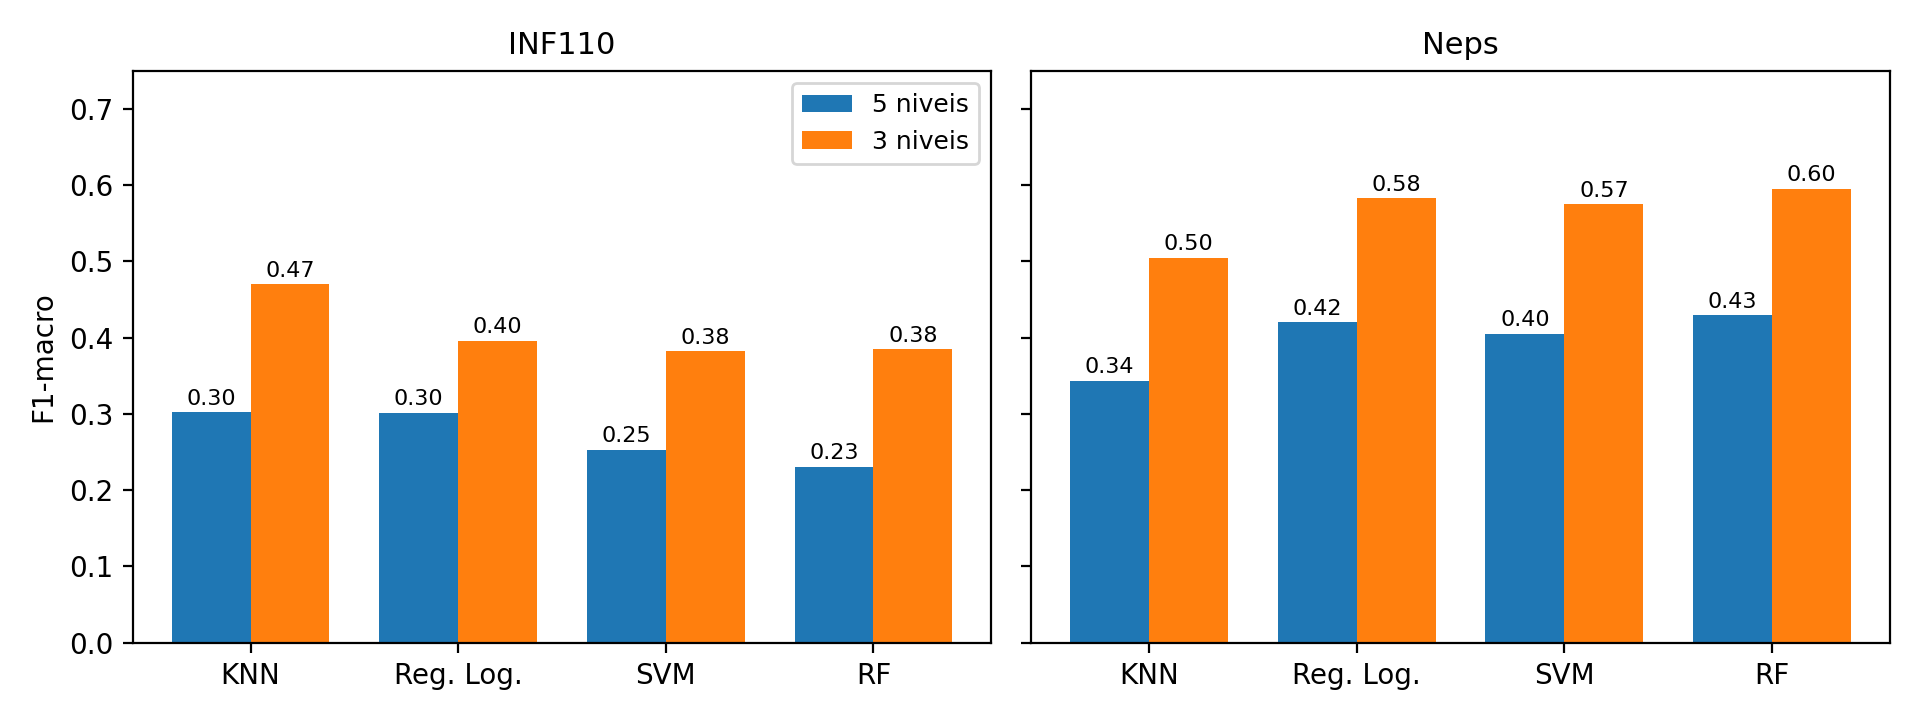
\includegraphics[width=\linewidth]{comparacao_f1_consolidada}
  \caption{F1-macro por modelo, cinco \textit{versus} três níveis, nas duas bases. A escala de três níveis melhora o desempenho em todas as famílias e em ambas as bases; o Neps ultrapassa o INF110 nas duas granularidades.}
  \Description{Gráfico de barras com dois painéis (INF110 e Neps); em cada painel, quatro pares de barras (KNN, Reg. Log., SVM, RF) comparando 5 e 3 níveis. Todas as barras de 3 níveis são mais altas; as barras do Neps são mais altas que as do INF110.}
  \label{fig:barras}
\end{figure}

A Tabela~\ref{tab:resultados} consolida os quatro melhores modelos (um por combinação base/escala) contra o \textit{baseline}. O KNN é o melhor no INF110 nas duas escalas. No Neps, o Random Forest lidera, efeito do maior volume, que permite aos modelos de \textit{ensemble} explorarem interações não lineares.

\begin{table}[t]
  \caption{Melhor modelo por combinação base/escala, validação cruzada (5 partições). F1-macro reportado como média $\pm$ desvio-padrão.}
  \label{tab:resultados}
  \begin{tabular}{llccc}
    \toprule
    Base & Modelo & Acurácia & F1-macro & F1-pond. \\
    \midrule
    INF110 (5N) & KNN            & $0{,}425$ & $0{,}302 \pm 0{,}114$ & $0{,}398$ \\
    INF110 (3N) & KNN            & $0{,}488$ & $\mathbf{0{,}470} \pm 0{,}111$ & $0{,}474$ \\
    Neps   (5N) & Random Forest  & $0{,}546$ & $0{,}429 \pm 0{,}026$ & $0{,}528$ \\
    Neps   (3N) & Random Forest  & $0{,}644$ & $\mathbf{0{,}595} \pm 0{,}025$ & $0{,}635$ \\
    \midrule
    INF110 (5N) & \textit{Baseline}   & $0{,}350$ & $0{,}133$ & $0{,}185$ \\
    INF110 (3N) & \textit{Baseline}   & $0{,}475$ & $0{,}214$ & $0{,}307$ \\
    Neps   (5N) & \textit{Baseline}   & $0{,}422$ & $0{,}119$ & $0{,}250$ \\
    Neps   (3N) & \textit{Baseline}   & $0{,}494$ & $0{,}220$ & $0{,}326$ \\
    \bottomrule
  \end{tabular}
\end{table}

\subsection{O Que a Matriz de Confusão Revela}
\label{sec:matrizes}

A Figura~\ref{fig:matrizes} traz, em uma única figura, as quatro matrizes de confusão \textit{out-of-fold} correspondentes aos melhores modelos. Ler o painel de cima para baixo, da esquerda para a direita, deixa claro o argumento em favor dos três níveis.

\begin{figure}[t]
  \centering
  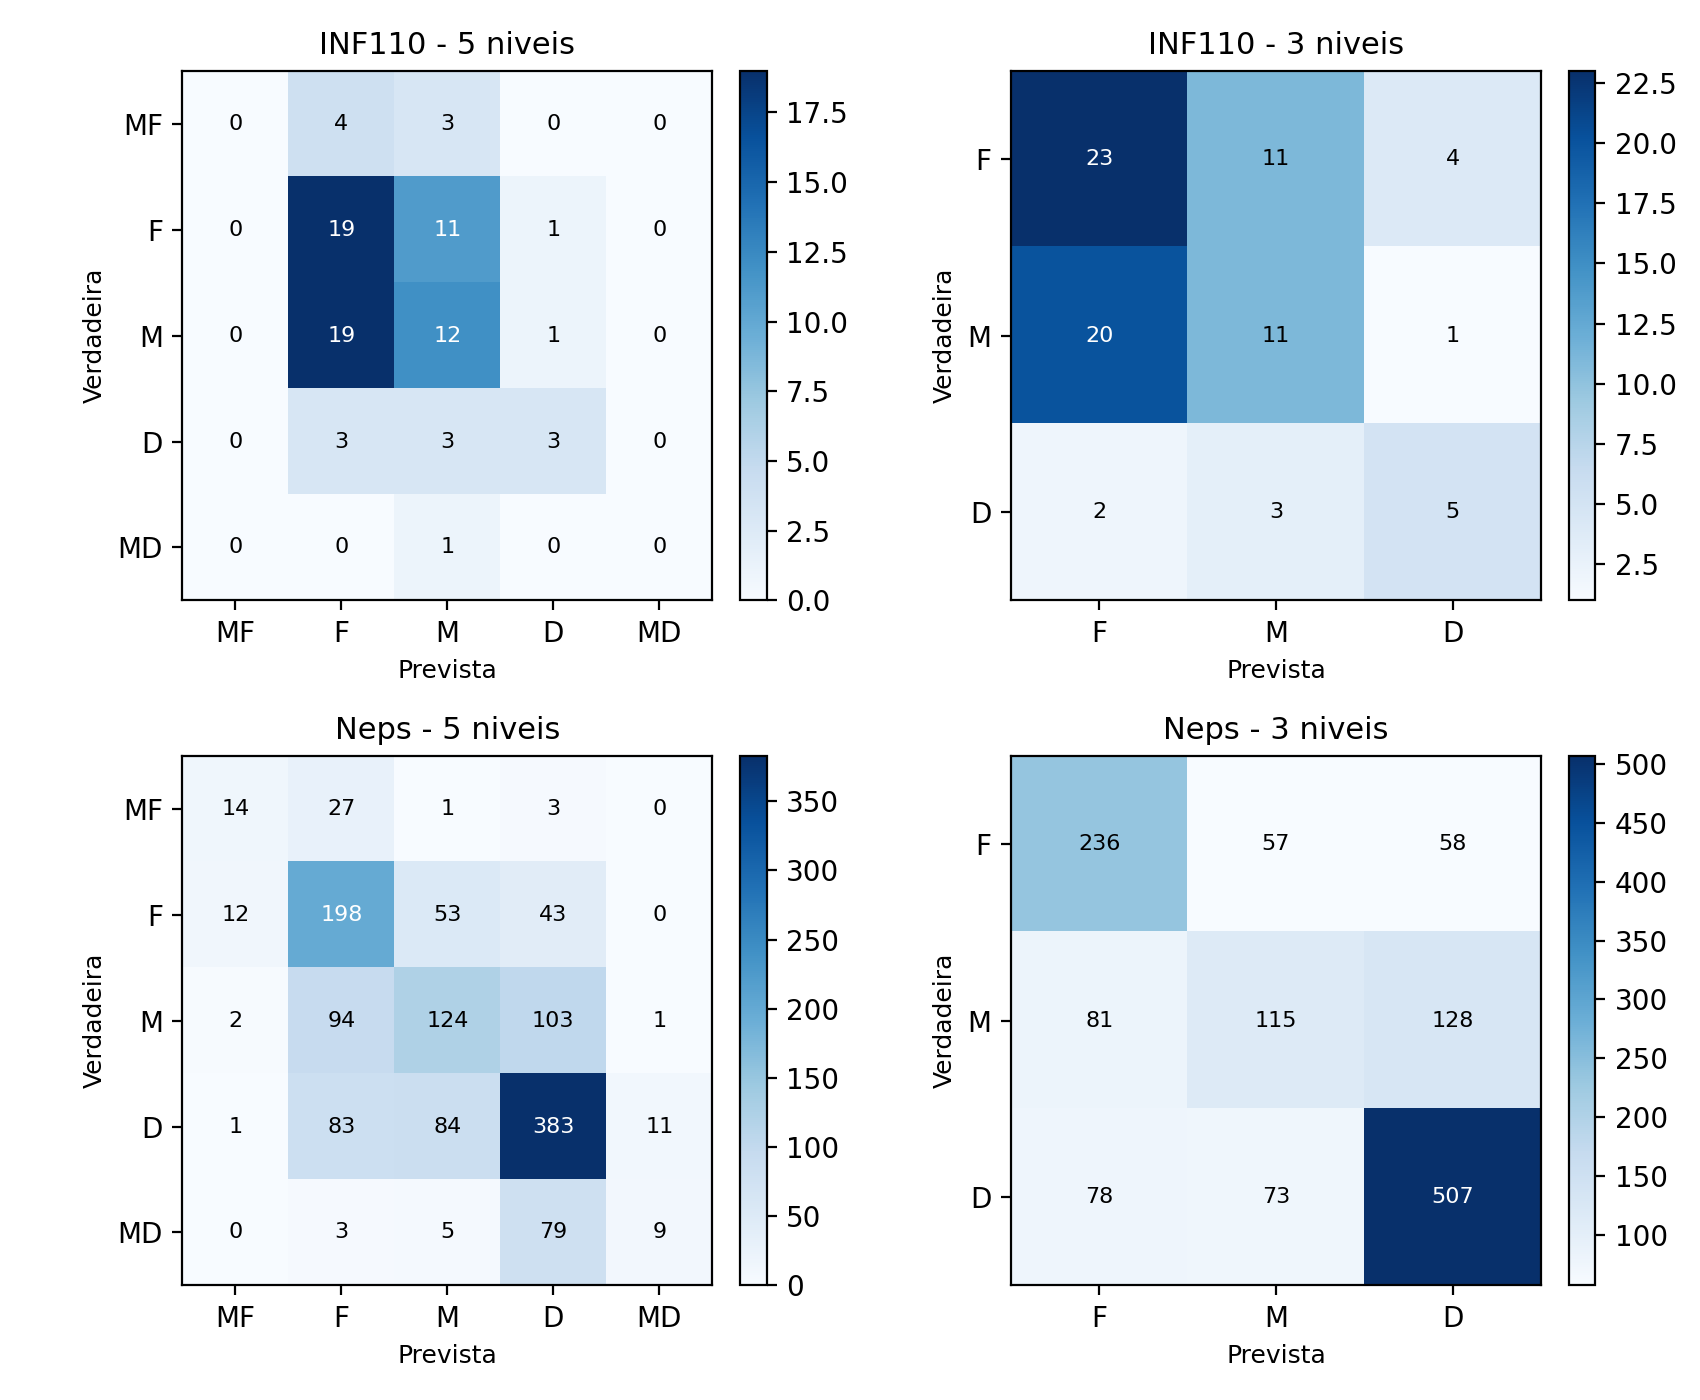
\includegraphics[width=\linewidth]{matrizes_consolidadas}
  \caption{Matrizes de confusão dos melhores modelos, com predições \textit{out-of-fold}. Linhas: classe verdadeira; colunas: classe prevista. Painel superior: INF110 (5N à esquerda, 3N à direita). Painel inferior: Neps (5N à esquerda, 3N à direita).}
  \Description{Painel 2x2 de mapas de calor: em cima INF110 (5x5 e 3x3), em baixo Neps (5x5 e 3x3). Nas de 3 níveis, a diagonal é mais forte; no INF110-5N as colunas MF e MD estão vazias.}
  \label{fig:matrizes}
\end{figure}

No INF110 com cinco níveis (canto superior esquerdo), as colunas ``MF'' e ``MD'' \textbf{estão inteiramente vazias}: nenhuma questão foi classificada como muito fácil ou muito difícil, consequência direta de haver apenas 7 e 1 exemplos dessas classes. Ao colapsar para três níveis (canto superior direito), o problema desaparece: a classe ``difícil'' passa a receber 5 predições corretas e as três classes ficam efetivamente cobertas.

No Neps com cinco níveis (canto inferior esquerdo), o problema não é o mesmo. As classes extremas \textbf{são} previstas (14 acertos em MF, 9 em MD), graças ao volume maior. Ainda assim, há confusão significativa entre classes adjacentes, com 94 questões de nível médio classificadas como fáceis e 103 como difíceis. Ao passar para três níveis (canto inferior direito), a diagonal principal se fortalece, com destaque para 507 acertos em ``difícil''. Esse é o cenário do classificador em produção: Random Forest treinado no Neps em três níveis.

\subsection{Resposta à Pergunta de Pesquisa}
\label{sec:pergunta}

Recapitulando o percurso: começamos com a escala natural de cinco níveis nas duas bases e observamos que essa granularidade produz um modelo pouco útil no INF110 (classes extremas ausentes) e ainda limitado no Neps (confusão entre adjacentes). Ao colapsar para três níveis, todas as classes passaram a ser previstas e o F1-macro subiu de forma consistente, de $0{,}30$ para $0{,}47$ no INF110 e de $0{,}43$ para $0{,}60$ no Neps.

A resposta à pergunta de pesquisa é, portanto, \emph{parcialmente afirmativa}. Existe sinal aproveitável no enunciado textual, suficiente para uma classificação razoável na escala de \textbf{três níveis}, mas insuficiente na escala mais fina de cinco. O fator limitante predominante não é a escolha do modelo (as quatro famílias têm desempenho próximo), e sim a \textbf{granularidade do rótulo}, razão da opção pelos três níveis, somada à \textbf{quantidade e ao balanceamento dos dados rotulados}. A dificuldade percebida também depende de fatores externos ao texto (repertório prévio do aluno, familiaridade com paradigmas), o que estabelece um teto natural para abordagens puramente textuais.

\section{Código e Reprodutibilidade}
\label{sec:codigo}

Todo o código-fonte, a documentação (README com instruções passo a passo), os dados brutos e os artefatos intermediários (bases consolidadas, vetorizadores e modelos treinados) estão organizados em um repositório único e público, disponível em \url{https://github.com/<usuario>/TPFinal_INF420}\footnote{Substituir pelo link definitivo do repositório.}. O \textit{pipeline} é dividido em etapas independentes (ingestão, pré-processamento, treino, avaliação, extração de conceitos, recomendador, inferência), executáveis via linha de comando (\texttt{python -m src.<etapa>}), com configuração centralizada em um único arquivo \texttt{.env}. Todos os experimentos usam semente aleatória fixa, e o \textit{script} \texttt{rodar\_tudo.ps1} reproduz o relatório inteiro (INF110 e Neps, cinco e três níveis) do zero.

\section{Considerações Éticas}
\label{sec:etica}

Foram utilizados \textbf{modelos generativos} (LLMs, servidos pela plataforma Groq) em três papéis restritos e explicitamente documentados: (i) \textit{baseline} de classificação, para comparar contra os modelos clássicos; (ii) explicador da recomendação, gerando justificativas em linguagem natural sob demanda; e (iii) extrator de conceitos por enunciado. Nenhum uso do LLM envolve dados pessoais dos alunos: as \textbf{avaliações dos alunos do INF110 são anônimas} (apenas nota 1--5 por questão, sem identificação) e o LLM \emph{nunca} recebe informações de alunos --- apenas o texto do enunciado da questão. Também não há geração automatizada de decisões com impacto sobre pessoas: as saídas do sistema (dificuldade prevista e exercícios recomendados) são \emph{sugestões}, sem substituir o julgamento do professor. Estamos cientes de vieses potenciais no rótulo (percepção de alunos no INF110 tende a refletir o repertório médio da turma) e no LLM (modelos treinados com viés de vocabulário técnico em inglês), e os apresentamos abertamente no texto. As bibliotecas utilizadas (\texttt{scikit-learn}, \texttt{NLTK}, \texttt{OpenAI-compatible client}) têm licenças permissivas e são adequadamente citadas.

\section{Limitações e Lições Aprendidas}
\label{sec:limitacoes}

Entre os pontos fortes do trabalho estão a metodologia cuidadosa de avaliação (sem vazamento de informação, com \textit{baseline} de referência e validação cruzada estratificada), a modularidade do código, que suportou naturalmente a comparação entre duas bases muito diferentes, e a integração fim-a-fim de ML e LLM em uma única ferramenta prática.

As principais limitações também foram bem identificadas ao longo do desenvolvimento. O tamanho reduzido e o forte desbalanceamento do INF110 limitam o teto absoluto de desempenho e produzem desvios-padrão altos na validação cruzada. A escolha entre plataformas de LLM tem custo prático, pois deprecações e tetos de requisição mudam com frequência. O cliente OpenAI-compatível intercambiável reduz esse atrito, mas não o elimina. Além disso, comparar bases com semânticas de rótulo distintas (percepção do aluno na INF110 e juízo profissional no Neps) exigiu explicitar a não-equivalência dos alvos no texto para evitar leituras enganosas dos números.

Duas lições ficaram claras. A primeira é que a granularidade do rótulo pode ser uma decisão de modelagem tão relevante quanto a escolha do algoritmo, e por isso merece ser tratada como hiperparâmetro explícito, e não como convenção herdada da forma de coleta dos dados. A segunda é o valor de manter os experimentos plenamente reprodutíveis desde o começo. Semente aleatória fixa, pipeline em etapas independentes e artefatos versionados permitiram refazer a comparação inteira sempre que uma decisão foi revisitada.

\section{Conclusão e Trabalhos Futuros}
\label{sec:conclusao}

Este trabalho desenvolveu e avaliou um sistema reprodutível para classificação automática da dificuldade de questões de programação a partir do enunciado. Testamos empiricamente duas granularidades de rótulo (cinco e três níveis) em duas bases (INF110 e Neps Academy). A configuração final adota três níveis, escolha justificada pelo ganho consistente de precisão em todas as famílias de modelos e em ambas as bases. O melhor modelo atingiu F1-macro de $0{,}47$ no INF110 (KNN em três níveis) e de $0{,}60$ no Neps (Random Forest em três níveis). Este último é o classificador em produção.

Como trabalhos futuros, destacam-se: (i) a incorporação de \textit{embeddings} semânticos densos como representação alternativa ou complementar ao TF-IDF; (ii) a execução da comparação quantitativa completa com as abordagens baseadas em LLM, já suportada pelo arcabouço implementado; (iii) técnicas de mitigação de desbalanceamento, como reamostragem, ou a reformulação da tarefa como classificação ordinal; e (iv) a ampliação e o balanceamento da base de questões rotuladas, idealmente com avaliações de múltiplas instituições, para elevar o teto de desempenho alcançável.

\begin{acks}
Os autores agradecem ao professor da disciplina INF420 (Inteligência Artificial) da Universidade Federal de Viçosa pela orientação e pela disponibilização da base de dados de avaliações de dificuldade utilizada neste trabalho.
\end{acks}

\bibliographystyle{ACM-Reference-Format}
\bibliography{referencias}

\end{document}
